\begin{itemize}
\item{Explaining the tool}

\tab The Bayesian Belief and Decision Networks applet is a tool to visually solve Bayesian Nets. It has a robust variable elimination algorithm, and allows users to create their own networks and customize the domains and probabilities. The applet has features that allow the user to inspect probabilities, make observations, and monitor nodes. It also allows the user to manually do variable elimination and to inspect the factors created.\\ \footnote{http://www.aispace.org/bayes/help/general.shtml}

\tab The applet also has features to add no-forgetting arcs. There is an independence quiz mode that tests the user on his or her knowledge of the independence rules of Bayesian Nets.\\


\tab The applet can read an XML representation of a Bayesian Network called the XMLBIF format. The application version of the applet saves networks in this format\\

\tab The Verbose Query Window allows the user to manually execute variable elimination. It has a large canvas area to the right and a control panel on the left.\\

\tab During the "Eliminate Variables" stage, there are two ways in which you can choose variables to eliminate. The 'Auto-Eliminate' button will eliminate all the variables in the order specified by the heuristic which is specified by the drop down menu next to 'Heuristic:'. The available heuristics are 'Max-Cardinality', 'Min-Degree', 'Min-Factor', 'Min-Fill', 'Random', and 'Sequential'. The 'Eliminate Next' button will eliminate a single variable each time you press it. The second way to choose variables to eliminate is by clicking on them directly. When you eliminate a variable, it will be greyed out, and the lists of current and eliminated factors will be updated accordingly. \\\footnote{http://www.aispace.org/bayes/help/general.shtml}


\item Algorithm of eliminating variables is:\\

\begin{center}
  	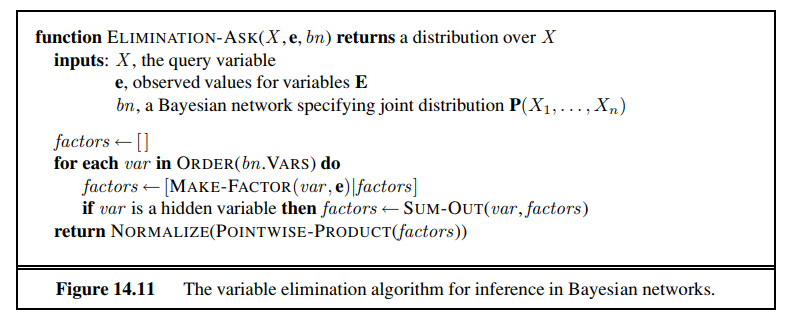
\includegraphics[scale=0.5]{eliminateVar}
\end{center}

\end{itemize}